% Options for packages loaded elsewhere
\PassOptionsToPackage{unicode}{hyperref}
\PassOptionsToPackage{hyphens}{url}
\PassOptionsToPackage{dvipsnames,svgnames,x11names}{xcolor}
%
\documentclass[
  a4paperpaper,
]{article}

\usepackage{amsmath,amssymb}
\usepackage{iftex}
\ifPDFTeX
  \usepackage[T1]{fontenc}
  \usepackage[utf8]{inputenc}
  \usepackage{textcomp} % provide euro and other symbols
\else % if luatex or xetex
  \ifXeTeX
    \usepackage{mathspec} % this also loads fontspec
  \else
    \usepackage{unicode-math} % this also loads fontspec
  \fi
  \defaultfontfeatures{Scale=MatchLowercase}
  \defaultfontfeatures[\rmfamily]{Ligatures=TeX,Scale=1}
\fi
\usepackage{lmodern}
\ifPDFTeX\else  
    % xetex/luatex font selection
\fi
% Use upquote if available, for straight quotes in verbatim environments
\IfFileExists{upquote.sty}{\usepackage{upquote}}{}
\IfFileExists{microtype.sty}{% use microtype if available
  \usepackage[]{microtype}
  \UseMicrotypeSet[protrusion]{basicmath} % disable protrusion for tt fonts
}{}
\makeatletter
\@ifundefined{KOMAClassName}{% if non-KOMA class
  \IfFileExists{parskip.sty}{%
    \usepackage{parskip}
  }{% else
    \setlength{\parindent}{0pt}
    \setlength{\parskip}{6pt plus 2pt minus 1pt}}
}{% if KOMA class
  \KOMAoptions{parskip=half}}
\makeatother
\usepackage{xcolor}
\setlength{\emergencystretch}{3em} % prevent overfull lines
\setcounter{secnumdepth}{-\maxdimen} % remove section numbering
% Make \paragraph and \subparagraph free-standing
\ifx\paragraph\undefined\else
  \let\oldparagraph\paragraph
  \renewcommand{\paragraph}[1]{\oldparagraph{#1}\mbox{}}
\fi
\ifx\subparagraph\undefined\else
  \let\oldsubparagraph\subparagraph
  \renewcommand{\subparagraph}[1]{\oldsubparagraph{#1}\mbox{}}
\fi

\usepackage{color}
\usepackage{fancyvrb}
\newcommand{\VerbBar}{|}
\newcommand{\VERB}{\Verb[commandchars=\\\{\}]}
\DefineVerbatimEnvironment{Highlighting}{Verbatim}{commandchars=\\\{\}}
% Add ',fontsize=\small' for more characters per line
\usepackage{framed}
\definecolor{shadecolor}{RGB}{241,243,245}
\newenvironment{Shaded}{\begin{snugshade}}{\end{snugshade}}
\newcommand{\AlertTok}[1]{\textcolor[rgb]{0.68,0.00,0.00}{#1}}
\newcommand{\AnnotationTok}[1]{\textcolor[rgb]{0.37,0.37,0.37}{#1}}
\newcommand{\AttributeTok}[1]{\textcolor[rgb]{0.40,0.45,0.13}{#1}}
\newcommand{\BaseNTok}[1]{\textcolor[rgb]{0.68,0.00,0.00}{#1}}
\newcommand{\BuiltInTok}[1]{\textcolor[rgb]{0.00,0.23,0.31}{#1}}
\newcommand{\CharTok}[1]{\textcolor[rgb]{0.13,0.47,0.30}{#1}}
\newcommand{\CommentTok}[1]{\textcolor[rgb]{0.37,0.37,0.37}{#1}}
\newcommand{\CommentVarTok}[1]{\textcolor[rgb]{0.37,0.37,0.37}{\textit{#1}}}
\newcommand{\ConstantTok}[1]{\textcolor[rgb]{0.56,0.35,0.01}{#1}}
\newcommand{\ControlFlowTok}[1]{\textcolor[rgb]{0.00,0.23,0.31}{#1}}
\newcommand{\DataTypeTok}[1]{\textcolor[rgb]{0.68,0.00,0.00}{#1}}
\newcommand{\DecValTok}[1]{\textcolor[rgb]{0.68,0.00,0.00}{#1}}
\newcommand{\DocumentationTok}[1]{\textcolor[rgb]{0.37,0.37,0.37}{\textit{#1}}}
\newcommand{\ErrorTok}[1]{\textcolor[rgb]{0.68,0.00,0.00}{#1}}
\newcommand{\ExtensionTok}[1]{\textcolor[rgb]{0.00,0.23,0.31}{#1}}
\newcommand{\FloatTok}[1]{\textcolor[rgb]{0.68,0.00,0.00}{#1}}
\newcommand{\FunctionTok}[1]{\textcolor[rgb]{0.28,0.35,0.67}{#1}}
\newcommand{\ImportTok}[1]{\textcolor[rgb]{0.00,0.46,0.62}{#1}}
\newcommand{\InformationTok}[1]{\textcolor[rgb]{0.37,0.37,0.37}{#1}}
\newcommand{\KeywordTok}[1]{\textcolor[rgb]{0.00,0.23,0.31}{#1}}
\newcommand{\NormalTok}[1]{\textcolor[rgb]{0.00,0.23,0.31}{#1}}
\newcommand{\OperatorTok}[1]{\textcolor[rgb]{0.37,0.37,0.37}{#1}}
\newcommand{\OtherTok}[1]{\textcolor[rgb]{0.00,0.23,0.31}{#1}}
\newcommand{\PreprocessorTok}[1]{\textcolor[rgb]{0.68,0.00,0.00}{#1}}
\newcommand{\RegionMarkerTok}[1]{\textcolor[rgb]{0.00,0.23,0.31}{#1}}
\newcommand{\SpecialCharTok}[1]{\textcolor[rgb]{0.37,0.37,0.37}{#1}}
\newcommand{\SpecialStringTok}[1]{\textcolor[rgb]{0.13,0.47,0.30}{#1}}
\newcommand{\StringTok}[1]{\textcolor[rgb]{0.13,0.47,0.30}{#1}}
\newcommand{\VariableTok}[1]{\textcolor[rgb]{0.07,0.07,0.07}{#1}}
\newcommand{\VerbatimStringTok}[1]{\textcolor[rgb]{0.13,0.47,0.30}{#1}}
\newcommand{\WarningTok}[1]{\textcolor[rgb]{0.37,0.37,0.37}{\textit{#1}}}

\providecommand{\tightlist}{%
  \setlength{\itemsep}{0pt}\setlength{\parskip}{0pt}}\usepackage{longtable,booktabs,array}
\usepackage{calc} % for calculating minipage widths
% Correct order of tables after \paragraph or \subparagraph
\usepackage{etoolbox}
\makeatletter
\patchcmd\longtable{\par}{\if@noskipsec\mbox{}\fi\par}{}{}
\makeatother
% Allow footnotes in longtable head/foot
\IfFileExists{footnotehyper.sty}{\usepackage{footnotehyper}}{\usepackage{footnote}}
\makesavenoteenv{longtable}
\usepackage{graphicx}
\makeatletter
\def\maxwidth{\ifdim\Gin@nat@width>\linewidth\linewidth\else\Gin@nat@width\fi}
\def\maxheight{\ifdim\Gin@nat@height>\textheight\textheight\else\Gin@nat@height\fi}
\makeatother
% Scale images if necessary, so that they will not overflow the page
% margins by default, and it is still possible to overwrite the defaults
% using explicit options in \includegraphics[width, height, ...]{}
\setkeys{Gin}{width=\maxwidth,height=\maxheight,keepaspectratio}
% Set default figure placement to htbp
\makeatletter
\def\fps@figure{htbp}
\makeatother

\usepackage{fvextra}
\DefineVerbatimEnvironment{Highlighting}{Verbatim}{breaklines,commandchars=\\\{\}}
\DefineVerbatimEnvironment{OutputCode}{Verbatim}{breaklines,commandchars=\\\{\}}
\makeatletter
\@ifpackageloaded{caption}{}{\usepackage{caption}}
\AtBeginDocument{%
\ifdefined\contentsname
  \renewcommand*\contentsname{Índice}
\else
  \newcommand\contentsname{Índice}
\fi
\ifdefined\listfigurename
  \renewcommand*\listfigurename{Lista de Figuras}
\else
  \newcommand\listfigurename{Lista de Figuras}
\fi
\ifdefined\listtablename
  \renewcommand*\listtablename{Lista de Tabelas}
\else
  \newcommand\listtablename{Lista de Tabelas}
\fi
\ifdefined\figurename
  \renewcommand*\figurename{Figura}
\else
  \newcommand\figurename{Figura}
\fi
\ifdefined\tablename
  \renewcommand*\tablename{Tabela}
\else
  \newcommand\tablename{Tabela}
\fi
}
\@ifpackageloaded{float}{}{\usepackage{float}}
\floatstyle{ruled}
\@ifundefined{c@chapter}{\newfloat{codelisting}{h}{lop}}{\newfloat{codelisting}{h}{lop}[chapter]}
\floatname{codelisting}{Listagem}
\newcommand*\listoflistings{\listof{codelisting}{Lista de Listagens}}
\makeatother
\makeatletter
\makeatother
\makeatletter
\@ifpackageloaded{caption}{}{\usepackage{caption}}
\@ifpackageloaded{subcaption}{}{\usepackage{subcaption}}
\makeatother
\ifLuaTeX
\usepackage[bidi=basic]{babel}
\else
\usepackage[bidi=default]{babel}
\fi
\babelprovide[main,import]{portuguese}
% get rid of language-specific shorthands (see #6817):
\let\LanguageShortHands\languageshorthands
\def\languageshorthands#1{}
\ifLuaTeX
  \usepackage{selnolig}  % disable illegal ligatures
\fi
\usepackage{bookmark}

\IfFileExists{xurl.sty}{\usepackage{xurl}}{} % add URL line breaks if available
\urlstyle{same} % disable monospaced font for URLs
\hypersetup{
  pdftitle={Lista 1: Ajustando uma RNA `no braço'},
  pdfauthor={César A. Galvão - 190011572},
  pdflang={pt},
  colorlinks=true,
  linkcolor={blue},
  filecolor={Maroon},
  citecolor={Blue},
  urlcolor={Blue},
  pdfcreator={LaTeX via pandoc}}

\title{Lista 1: Ajustando uma RNA `no braço'}
\author{César A. Galvão - 190011572}
\date{}

\begin{document}
\maketitle

Para essa lista, é considerada a seguinte arquitetura de uma rede neural
\emph{feed-forward}:

\begin{figure}[H]

{\centering 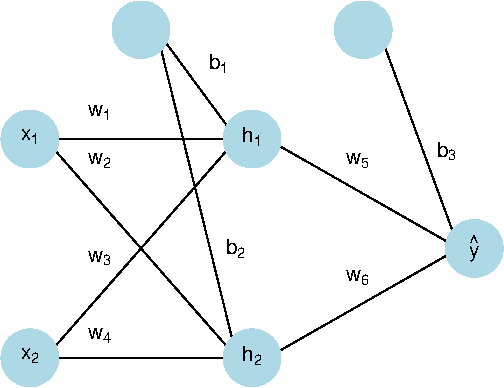
\includegraphics{lista1-resolucao_files/figure-pdf/figf-arquitetura-rede-1.pdf}

}

\caption{Arquitetura da rede neural artificial. Adotamos função de
ativação sigmoide e linear nas camadas escondidas e de saída,
respectivamente.}

\end{figure}%

\section{Questão 1}\label{questuxe3o-1}

\subsection{Item a}\label{item-a}

Crie uma função computacional para calcular o valor previso da variável
resposta \(\hat{y} = f(\boldsymbol{x}; \boldsymbol{\theta})\) em função
de \(\boldsymbol{x}\) e \(\boldsymbol{\theta}\). Use a função para
calcular \(\hat{y}\) para \(\boldsymbol{\theta} = (0.1, \dots , 0.1)\) e
\(\boldsymbol{x} = (1, 1)\).

\begin{center}\rule{0.5\linewidth}{0.5pt}\end{center}

Implementa-se de forma matricial. A função não é adaptativa ao tamanho
da rede e exige que o usuário forneça uma lista \(\boldsymbol{\theta}\)
com os seguintes elementos:

\begin{enumerate}
\def\labelenumi{\arabic{enumi}.}
\tightlist
\item
  \(W^{(1)}\) - matriz \(2 \times 2\) de pesos da camada de entrada
  \(\begin{pmatrix} w_1 & w_2 \\ w_3 & w_4 \end{pmatrix}\). Cada linha
  deve representar os pesos de cada neurônio para o neurônio
  subsequente, i.e.~\(w_{ij}\) representa o peso do neurônio de entrada
  \(i\) para o próximo neurônio \(j\).
\item
  \(\boldsymbol{b}^{(1)}\) - vetor de viés da camada de entrada
  \(\begin{pmatrix} b_1 \\ b_2 \end{pmatrix}\).
\item
  \(W^{(2)}\) - matriz \(2 \times 1\) de pesos da camada de saída
  \(\begin{pmatrix} w_5 \\ w_6 \end{pmatrix}\).
\item
  \(\boldsymbol{b}^{(2)}\) - vetor elemento de viés da camada de saída
  \(\begin{pmatrix} b_3 \end{pmatrix}\).
\end{enumerate}

Como função de ativação foi escolhida a função sigmóide denotada por
\(\phi = \frac{1}{1+e^{-x}}\). A função de previsão é dada por:

\[
\hat{y} = W^{(2)\top}\phi(W^{(1)\top}\boldsymbol{x} + \boldsymbol{b}^{(1)}) + \boldsymbol{b}^{(2)}
\]

ou

\begin{align*}
\boldsymbol{a} =& W^{(1)\top} \boldsymbol{x} + \boldsymbol{b^{(1)}} \\
\boldsymbol{h} =& \phi(\boldsymbol{a}) \\
\hat{y} =& W^{(2)\top}\boldsymbol{h} + b^{(2)}
\end{align*}

\begin{Shaded}
\begin{Highlighting}[]
\CommentTok{\# Função de ativação}
\NormalTok{phi }\OtherTok{\textless{}{-}} \ControlFlowTok{function}\NormalTok{(x) \{}\DecValTok{1}\SpecialCharTok{/}\NormalTok{(}\DecValTok{1} \SpecialCharTok{+} \FunctionTok{exp}\NormalTok{(}\SpecialCharTok{{-}}\NormalTok{x))\}}

\CommentTok{\# Função de previsão}
\NormalTok{ffwd }\OtherTok{\textless{}{-}} \ControlFlowTok{function}\NormalTok{(x, theta) \{}
  
  \ControlFlowTok{if}\NormalTok{(}\FunctionTok{any}\NormalTok{(}\FunctionTok{dim}\NormalTok{(theta[[}\DecValTok{1}\NormalTok{]]) }\SpecialCharTok{!=} \FunctionTok{c}\NormalTok{(}\DecValTok{2}\NormalTok{, }\DecValTok{2}\NormalTok{)))\{}
    \FunctionTok{stop}\NormalTok{(}\StringTok{"O primeiro elemento de theta deve ser uma matriz de pesos 2x2 para a aplicação nos dados"}\NormalTok{)}
\NormalTok{  \} }\ControlFlowTok{else} \ControlFlowTok{if}\NormalTok{(}\FunctionTok{length}\NormalTok{(theta[[}\DecValTok{2}\NormalTok{]]) }\SpecialCharTok{!=} \DecValTok{2}\NormalTok{)\{}
    \FunctionTok{stop}\NormalTok{(}\StringTok{"O segundo elemento de theta deve ser um vetor viés de tamanho 2 para somar aos dados"}\NormalTok{)}
\NormalTok{  \} }\ControlFlowTok{else} \ControlFlowTok{if}\NormalTok{(}\FunctionTok{any}\NormalTok{(}\FunctionTok{dim}\NormalTok{(theta[[}\DecValTok{3}\NormalTok{]]) }\SpecialCharTok{!=} \FunctionTok{c}\NormalTok{(}\DecValTok{2}\NormalTok{, }\DecValTok{1}\NormalTok{)))\{}
    \FunctionTok{stop}\NormalTok{(}\StringTok{"O terceiro elemento de theta deve ser uma matriz de pesos 2x1 para aplicação na única camada h"}\NormalTok{)}
\NormalTok{  \} }\ControlFlowTok{else} \ControlFlowTok{if}\NormalTok{(}\FunctionTok{length}\NormalTok{(theta[[}\DecValTok{4}\NormalTok{]]) }\SpecialCharTok{!=} \DecValTok{1}\NormalTok{)\{}
    \FunctionTok{stop}\NormalTok{(}\StringTok{"O quarto elemento de theta deve ser um vetor viés de tamanho 1 para soma na única camada h"}\NormalTok{)}
\NormalTok{  \} }\ControlFlowTok{else} \ControlFlowTok{if}\NormalTok{(}\SpecialCharTok{!}\FunctionTok{is.vector}\NormalTok{(x) }\SpecialCharTok{\&} \FunctionTok{length}\NormalTok{(x) }\SpecialCharTok{!=} \DecValTok{2}\NormalTok{)\{}
    \FunctionTok{stop}\NormalTok{(}\StringTok{"O x deve ser um vetor de tamanho 2"}\NormalTok{)}
\NormalTok{  \}}
  
\NormalTok{  x }\OtherTok{\textless{}{-}} \FunctionTok{as.vector}\NormalTok{(x)}
  
\NormalTok{  W1 }\OtherTok{\textless{}{-}}\NormalTok{ theta[[}\DecValTok{1}\NormalTok{]]}
\NormalTok{  b1 }\OtherTok{\textless{}{-}}\NormalTok{ theta[[}\DecValTok{2}\NormalTok{]]}
\NormalTok{  W2 }\OtherTok{\textless{}{-}}\NormalTok{ theta[[}\DecValTok{3}\NormalTok{]]}
\NormalTok{  b2 }\OtherTok{\textless{}{-}}\NormalTok{ theta[[}\DecValTok{4}\NormalTok{]]}
  
\NormalTok{  a1 }\OtherTok{\textless{}{-}}\NormalTok{ (}\FunctionTok{t}\NormalTok{(W1)}\SpecialCharTok{\%*\%}\NormalTok{x)}\SpecialCharTok{+}\NormalTok{b1}
\NormalTok{  h }\OtherTok{\textless{}{-}} \FunctionTok{phi}\NormalTok{(a1)}
\NormalTok{  yhat }\OtherTok{\textless{}{-}}\NormalTok{ (}\FunctionTok{t}\NormalTok{(W2)}\SpecialCharTok{\%*\%}\NormalTok{h)}\SpecialCharTok{+}\NormalTok{b2}
  
  \FunctionTok{return}\NormalTok{( }\CommentTok{\# separacao dos elementos de saída para usar no backpropagation}
    \FunctionTok{list}\NormalTok{(}\AttributeTok{yhat =} \FunctionTok{as.double}\NormalTok{(yhat),}
         \AttributeTok{hidden =}\NormalTok{ h,}
         \AttributeTok{pre\_activation =}\NormalTok{ a1)}
\NormalTok{  )}
\NormalTok{\}}
\end{Highlighting}
\end{Shaded}

~

Agora vamos calcular \(\hat{y}\) para
\(\boldsymbol{\theta} = (0.1, \dots , 0.1)\) e
\(\boldsymbol{x} = (1, 1)\).

\begin{Shaded}
\begin{Highlighting}[]
\NormalTok{x }\OtherTok{\textless{}{-}} \FunctionTok{c}\NormalTok{(}\DecValTok{1}\NormalTok{,}\DecValTok{1}\NormalTok{)}

\NormalTok{theta }\OtherTok{\textless{}{-}} \FunctionTok{list}\NormalTok{(}
  \FunctionTok{matrix}\NormalTok{(}\FunctionTok{c}\NormalTok{(}\FloatTok{0.1}\NormalTok{), }\AttributeTok{nrow =} \DecValTok{2}\NormalTok{, }\AttributeTok{ncol =} \DecValTok{2}\NormalTok{), }\CommentTok{\#w1}
  \FunctionTok{c}\NormalTok{(}\FloatTok{0.1}\NormalTok{, }\FloatTok{0.1}\NormalTok{), }\CommentTok{\#b1}
  \FunctionTok{matrix}\NormalTok{(}\FunctionTok{c}\NormalTok{(}\FloatTok{0.1}\NormalTok{), }\AttributeTok{nrow =} \DecValTok{2}\NormalTok{, }\AttributeTok{ncol =} \DecValTok{1}\NormalTok{), }\CommentTok{\#w2}
  \FunctionTok{c}\NormalTok{(}\FloatTok{0.1}\NormalTok{) }\CommentTok{\#b2}
\NormalTok{)}

\FunctionTok{ffwd}\NormalTok{(x, theta)}
\end{Highlighting}
\end{Shaded}

Obtemos \(\hat{y} =\) 0.2148885.

\subsection{Item b}\label{item-b}

Crie uma rotina computacional para calcular a função de custo
\(J(\theta)\). Em seguida, divida o conjunto de dados observados de modo
que as \textbf{primeiras} \(80.000\) amostras componham o conjunto de
\textbf{treinamento}, as próximas \(10.000\) o de \textbf{validação}, e
as \textbf{últimas} \(10.000\) o de \textbf{teste}. Qual é o custo da
rede no \textbf{conjunto de teste} quando
\(\boldsymbol{\theta} = (0.1, . . . , 0.1)\)?

\begin{center}\rule{0.5\linewidth}{0.5pt}\end{center}

Primeiro são gerados os dados conforme as instruções da lista:

\begin{Shaded}
\begin{Highlighting}[]
\DocumentationTok{\#\#\# Gerando dados "observados"}
\FunctionTok{set.seed}\NormalTok{(}\FloatTok{1.2024}\NormalTok{)}
\NormalTok{m.obs }\OtherTok{\textless{}{-}} \DecValTok{100000}
\NormalTok{dados }\OtherTok{\textless{}{-}} \FunctionTok{tibble}\NormalTok{(}\AttributeTok{x1.obs=}\FunctionTok{runif}\NormalTok{(m.obs, }\SpecialCharTok{{-}}\DecValTok{3}\NormalTok{, }\DecValTok{3}\NormalTok{),}
                \AttributeTok{x2.obs=}\FunctionTok{runif}\NormalTok{(m.obs, }\SpecialCharTok{{-}}\DecValTok{3}\NormalTok{, }\DecValTok{3}\NormalTok{)) }\SpecialCharTok{\%\textgreater{}\%}
         \FunctionTok{mutate}\NormalTok{(}\AttributeTok{mu=}\FunctionTok{abs}\NormalTok{(x1.obs}\SpecialCharTok{\^{}}\DecValTok{3} \SpecialCharTok{{-}} \DecValTok{30}\SpecialCharTok{*}\FunctionTok{sin}\NormalTok{(x2.obs) }\SpecialCharTok{+} \DecValTok{10}\NormalTok{), }
                \AttributeTok{y=}\FunctionTok{rnorm}\NormalTok{(m.obs, }\AttributeTok{mean=}\NormalTok{mu, }\AttributeTok{sd=}\DecValTok{1}\NormalTok{))}
\end{Highlighting}
\end{Shaded}

~

Depois, implementamos a função de custo \(J(\theta)\), que é dada por

\begin{align*}
  J(\boldsymbol{\theta}) =& \frac{1}{m}\sum\limits_{i = 1}^{m} L \left( f(x_{1i}, x_{2i}; \boldsymbol{\theta}), y_i \right) \\ 
  =& \frac{1}{m}\sum\limits_{i = 1}^{m} \left( f(x_{1i}, x_{2i}; \boldsymbol{\theta}) - y_i \right)^2 \\ 
  =& \frac{1}{m}\sum\limits_{i = 1}^{m} \left( \hat{y}_i - y_i \right)^2,
\end{align*}

onde \(m\) é o número de observações.

\begin{Shaded}
\begin{Highlighting}[]
\NormalTok{J.Loss }\OtherTok{\textless{}{-}} \ControlFlowTok{function}\NormalTok{(dados, theta, target)\{}
  
  \ControlFlowTok{if}\NormalTok{(}\SpecialCharTok{!}\FunctionTok{is.data.frame}\NormalTok{(dados) }\SpecialCharTok{|} \SpecialCharTok{!}\FunctionTok{is\_tibble}\NormalTok{(dados))\{}
    \FunctionTok{stop}\NormalTok{(}\StringTok{"Dados deve ser uma dataframe ou tibble."}\NormalTok{)}
\NormalTok{  \} }\ControlFlowTok{else} \ControlFlowTok{if}\NormalTok{ (}\FunctionTok{dim}\NormalTok{(dados)[}\DecValTok{2}\NormalTok{] }\SpecialCharTok{!=} \DecValTok{2}\NormalTok{)\{}
    \FunctionTok{stop}\NormalTok{(}\StringTok{"Matriz de dados deve ter 2 colunas."}\NormalTok{)}
\NormalTok{  \} }\ControlFlowTok{else} \ControlFlowTok{if}\NormalTok{ (}\SpecialCharTok{!}\FunctionTok{is.list}\NormalTok{(theta))\{}
    \FunctionTok{stop}\NormalTok{(}\StringTok{"Theta deve ser uma lista com pesos e viéses."}\NormalTok{)}
\NormalTok{  \} }\ControlFlowTok{else} \ControlFlowTok{if}\NormalTok{ (}\SpecialCharTok{!}\FunctionTok{is.numeric}\NormalTok{(target))\{}
    \FunctionTok{stop}\NormalTok{(}\StringTok{"Target deve ser um vetor numérico."}\NormalTok{)}
\NormalTok{  \}}
  
\CommentTok{\# aloca memoria para o tamanho dos dados}
\NormalTok{  yhat }\OtherTok{\textless{}{-}} \FunctionTok{double}\NormalTok{(}\FunctionTok{nrow}\NormalTok{(dados))}
\CommentTok{\# transpoe os dados para termos acesso aos vetores de x que serao passados para a primeira camada da rede}
\NormalTok{  tdados }\OtherTok{\textless{}{-}} \FunctionTok{t}\NormalTok{(}\FunctionTok{as.matrix}\NormalTok{(dados))}
  
  \ControlFlowTok{for}\NormalTok{(i }\ControlFlowTok{in} \DecValTok{1}\SpecialCharTok{:}\FunctionTok{ncol}\NormalTok{(tdados))\{}
\NormalTok{    yhat[i] }\OtherTok{\textless{}{-}} \FunctionTok{ffwd}\NormalTok{(tdados[,i], theta)}\SpecialCharTok{$}\NormalTok{yhat}
\NormalTok{  \}}
  
  \FunctionTok{return}\NormalTok{(}\FunctionTok{mean}\NormalTok{((target }\SpecialCharTok{{-}}\NormalTok{ yhat)}\SpecialCharTok{\^{}}\DecValTok{2}\NormalTok{)) }\CommentTok{\#média ja entrega soma/m}
  
\NormalTok{\}}
\end{Highlighting}
\end{Shaded}

~

Em seguida, separamos o nosso conjunto de dados em treinamento,
validação e teste.

\begin{Shaded}
\begin{Highlighting}[]
\NormalTok{dados\_train }\OtherTok{\textless{}{-}}\NormalTok{ dados[}\DecValTok{1}\SpecialCharTok{:}\DecValTok{80000}\NormalTok{,]}
\NormalTok{dados\_valid }\OtherTok{\textless{}{-}}\NormalTok{ dados[}\DecValTok{80001}\SpecialCharTok{:}\DecValTok{90000}\NormalTok{,]}
\NormalTok{dados\_test }\OtherTok{\textless{}{-}}\NormalTok{ dados[}\DecValTok{90001}\SpecialCharTok{:}\FunctionTok{nrow}\NormalTok{(dados),]}
\end{Highlighting}
\end{Shaded}

~

Finalmente, executamos a função de \emph{feed-forward} nos dados gerados
para calcularmos \(\boldsymbol{\hat{y}}\) e em seguida calculamos o
custo da rede com \(\boldsymbol{\theta} = (0.1, \dots, 0.1)\).

\begin{Shaded}
\begin{Highlighting}[]
\CommentTok{\# transformamos os dados em matriz}
\NormalTok{x\_test }\OtherTok{\textless{}{-}}\NormalTok{ dados\_test }\SpecialCharTok{\%\textgreater{}\%} 
  \FunctionTok{select}\NormalTok{(x1.obs, x2.obs)}

\CommentTok{\# separamos o target}
\NormalTok{y\_test }\OtherTok{\textless{}{-}}\NormalTok{ dados\_test }\SpecialCharTok{\%\textgreater{}\%}
  \FunctionTok{pull}\NormalTok{(y)}

\CommentTok{\# theta já foi gerado e será reaproveitado}
\FunctionTok{J.Loss}\NormalTok{(x\_test, theta, y\_test)}
\end{Highlighting}
\end{Shaded}

~

Obtemos um custo de 663.1286383.

\subsection{Item c}\label{item-c}

Use a regra da cadeia para encontrar expressões algébricas para o vetor
gradiente

\[
\nabla_{\boldsymbol{\theta}}J(\boldsymbol{\theta}) = \left( \frac{\partial J}{\partial w_1}, \dots, \frac{\partial J}{\partial b_3} \right).
\]

\begin{center}\rule{0.5\linewidth}{0.5pt}\end{center}

Desejamos \(\nabla_{\boldsymbol{\theta}}J(\boldsymbol{\theta})\) tal que

\begin{align}
  \nabla_{\boldsymbol{\theta}}J(\boldsymbol{\theta}) &= \nabla_{\boldsymbol{\theta}} \left[ \frac{1}{m} \sum\limits^m_{i = 1} (y - \hat{y}_i)^2 \right] \nonumber \\
  &= \frac{2}{m} \sum\limits^m_{i = 1} (y - \hat{y}_i) \nabla_{\boldsymbol{\theta}} (y - \hat{y}_i), \quad \text{pois } \hat{y}_i = f(x_{1i}, x_{2i}; \boldsymbol{\theta}) \nonumber \\
  &= \frac{2}{m} \sum\limits^m_{i = 1} (y - \hat{y}_i) (-1) \nabla_{\boldsymbol{\theta}} \hat{y}_i \label{101}
\end{align}

Resolvemos o gradiente, considerando
\(\phi(x) = \sigma(x) = \frac{1}{1+ e^{-x}}\),

\begin{align*}
  \nabla_{\boldsymbol{\theta}} \hat{y}_i &= \nabla_{\boldsymbol{\theta}} \left[ h_{1i} w_5 + h_{2i} w_6 + b_3 \right] \\
  &= \nabla_{\boldsymbol{\theta}} \left[ \phi(a_{1i}) w_5 + \phi(a_{2i}) w_6 + b_3 \right] \\
  &= \nabla_{\boldsymbol{\theta}} \left[ \phi(x_{1i} w_1 + x_{2i} w_3 + b_1) w_5 + \phi(x_{1i} w_2 + x_{2i} w_4 + b_2) w_6 + b_3 \right].
\end{align*}

É imediato que

\begin{align*}
  \frac{\partial \hat{y}_i}{\partial b_3} = 1, \quad \frac{\partial \hat{y}_i}{\partial w_5} = h_{1i}, \quad \frac{\partial \hat{y}_i}{\partial w_6} = h_{2i}.
\end{align*}

Para \(b_j, j \in \{1, 2\}\) resolvemos de forma análoga:

\begin{align*}
\frac{\partial \hat{y}_i}{\partial b_1} &= w_5 \frac{\partial h_1}{\partial b_1} = w_5 \frac{\partial}{\partial b_1} \phi(x_{1i} w_1 + x_{2i} w_3 + b_1) \\  
&= w_5 \frac{\partial}{\partial b_1} \left( \frac{1}{1+ e^{-(x_{1i} w_1 + x_{2i} w_3 + b_1)}} \right) \\  
&= w_5 \frac{(-1) \cdot \frac{\partial}{\partial b_1} \left(1+ e^{-(x_{1i} w_1 + x_{2i} w_3 + b_1)} \right)}{\left(1+ e^{-(x_{1i} w_1 + x_{2i} w_3 + b_1)} \right)^2}
\end{align*}

e

\begin{align*}
\frac{\partial}{\partial b_1} \left(1+ e^{x_{1i} w_1 + x_{2i} w_3 + b_1} \right) &= 1 \cdot e^{x_{1i} w_1 + x_{2i} w_3 + b_1} \\
&= e^{x_{1i} w_1 + x_{2i} w_3 + b_1} = e^{a_1}.
\end{align*}

Portanto,

\begin{align*}
  \frac{\partial \hat{y}_i}{\partial b_1} &= w_5 \frac{-e^{a_1}}{\left( 1+e^{a_1} \right)^2 }, \quad \text{e } \quad \frac{\partial \hat{y}_i}{\partial b_2} = w_6 \frac{-e^{a_2}}{\left( 1+e^{a_2} \right)^2 }.
\end{align*}

Para \(w_j, j \in \{ 1, 2, 3, 4 \}\),

\begin{align*}
  \frac{\partial \hat{y}_i}{\partial w_1} &= w_5 \frac{\partial h_1}{\partial w_1} = w_5 \frac{-x_{1i} \, e^{a_1}}{\left(1 + e^{a_1}\right)^2} \\
  \frac{\partial \hat{y}_i}{\partial w_2} &= w_6 \frac{-x_{1i} \, e^{a_2}}{\left(1 + e^{a_2}\right)^2} \\
  \frac{\partial \hat{y}_i}{\partial w_3} &= w_5 \frac{-x_{2i} \, e^{a_1}}{\left(1 + e^{a_1}\right)^2} \\
  \frac{\partial \hat{y}_i}{\partial w_4} &= w_6 \frac{-x_{2i} \, e^{a_2}}{\left(1 + e^{a_2}\right)^2}.
\end{align*}

Finalmente, substituimos os as componentes na equação (\ref{101}) e
explicitamos cada componente do gradiente\footnote{Essa notação poderia
  ser escrita de forma mais elegante e sucinta. No entanto, dessa forma
  facilita a comparação entre a expressão analítica e a implementação
  computacional pelo leitor.}:

\begin{align}
  \nabla_{\boldsymbol{\theta}}J(\boldsymbol{\theta}) = \begin{pmatrix}
% MATRIZ SIMPLIFICADA
\frac{\partial J}{\partial w_1} \\ \\
\frac{\partial J}{\partial w_2} \\ \\
\frac{\partial J}{\partial w_3} \\ \\
\frac{\partial J}{\partial w_4} \\ \\
\frac{\partial J}{\partial w_5} \\ \\
\frac{\partial J}{\partial w_6} \\ \\
\frac{\partial J}{\partial b_1} \\ \\
\frac{\partial J}{\partial b_2} \\ \\
\frac{\partial J}{\partial b_3} \end{pmatrix} = \begin{pmatrix} 
% MATRIZ EXPLÍCITA
\frac{2}{m} \sum\limits^m_{i = 1}(y - \hat{y}_i) \, w_5 \, x_{1i} \frac{e^{a_{1i}}}{(1+e^{a_{1i}})^2} \\ \\ 
\frac{2}{m} \sum\limits^m_{i = 1}(y - \hat{y}_i) \, w_6 \, x_{1i} \frac{e^{a_{2i}}}{(1+e^{a_{2i}})^2} \\ \\ 
\frac{2}{m} \sum\limits^m_{i = 1}(y - \hat{y}_i) \, w_5 \, x_{2i} \frac{e^{a_{1i}}}{(1+e^{a_{1i}})^2} \\ \\ 
\frac{2}{m} \sum\limits^m_{i = 1}(y - \hat{y}_i) \, w_6 \, x_{2i} \frac{e^{a_{2i}}}{(1+e^{a_{2i}})^2} \\ \\ 
\frac{2}{m} \sum\limits^m_{i = 1}(y - \hat{y}_i) \, (-h_{1i}) \\ \\ 
\frac{2}{m} \sum\limits^m_{i = 1}(y - \hat{y}_i) \, (-h_{2i}) \\ \\ 
\frac{2}{m} \sum\limits^m_{i = 1}(y - \hat{y}_i) \, w_5 \frac{e^{a_{1i}}}{(1+e^{a_{1i}})^2} \\ \\ 
\frac{2}{m} \sum\limits^m_{i = 1}(y - \hat{y}_i) \, w_6 \frac{e^{a_{2i}}}{(1+e^{a_{2i}})^2} \\ \\ 
\frac{2}{m} \sum\limits^m_{i = 1}(y - \hat{y}_i)(-1)
\end{pmatrix}
\end{align}  

~

\subsection{Item d}\label{item-d}

Crie uma função computacional que receba como entrada o vetor
\(\theta\), uma matriz design \((x)\) e as respectivas observações
\((y)\) e forneça, como saída, o gradiente definido no item c).
Apresente o resultado da função aplicada sobre o banco de treinamento,
quando \(\theta = (0.1, \dots , 0.1)\). Atenção: implemente o algoritmo
\emph{back-propagation} (Algoritmo 6.4 do livro Deep Learning) para
evitar realizar a mesma operação múltiplas vezes.

\begin{center}\rule{0.5\linewidth}{0.5pt}\end{center}

na função, para responder de D a F:

function(theta, dados, target, optimize = TRUE, learning\_rate = NULL,
epochs = NULL, plot = FALSE)

\begin{itemize}
\tightlist
\item
  optimize: se true, otimiza. Se false, retorna o gradiente. padrao é
  true.
\item
  learning rate
\item
  iteracoes: numero de iteracoes
\item
  plot: se true, gera um elemento da lista de saída com o custo em cada
  iteracao. padrao é false.
\end{itemize}

\begin{Shaded}
\begin{Highlighting}[]
\NormalTok{backpropagation }\OtherTok{\textless{}{-}} \ControlFlowTok{function}\NormalTok{(theta, dados, target, }\AttributeTok{optimize =} \ConstantTok{TRUE}\NormalTok{, }\AttributeTok{learning\_rate =} \ConstantTok{NULL}\NormalTok{, }\AttributeTok{epochs =} \ConstantTok{NULL}\NormalTok{, }\AttributeTok{plot =} \ConstantTok{FALSE}\NormalTok{)\{}
  
  \ControlFlowTok{if}\NormalTok{(}\SpecialCharTok{!}\FunctionTok{is.list}\NormalTok{(theta))\{}
    \FunctionTok{stop}\NormalTok{(}\StringTok{"Theta deve ser uma lista com pesos e viéses."}\NormalTok{)}
\NormalTok{  \} }\ControlFlowTok{else} \ControlFlowTok{if}\NormalTok{(}\SpecialCharTok{!}\FunctionTok{is.data.frame}\NormalTok{(dados) }\SpecialCharTok{|} \SpecialCharTok{!}\FunctionTok{is.tibble}\NormalTok{(dados))\{}
    \FunctionTok{stop}\NormalTok{(}\StringTok{"Dados deve ser uma dataframe ou tibble."}\NormalTok{)}
\NormalTok{  \} }\ControlFlowTok{else} \ControlFlowTok{if}\NormalTok{(}\SpecialCharTok{!}\FunctionTok{is.numeric}\NormalTok{(target))\{}
    \FunctionTok{stop}\NormalTok{(}\StringTok{"Target deve ser um vetor numérico."}\NormalTok{)}
\NormalTok{  \} }\ControlFlowTok{else} \ControlFlowTok{if}\NormalTok{(}\SpecialCharTok{!}\FunctionTok{is.logical}\NormalTok{(optimize))\{}
    \FunctionTok{stop}\NormalTok{(}\StringTok{"Optimize deve ser um valor lógico."}\NormalTok{)}
\NormalTok{  \} }\ControlFlowTok{else} \ControlFlowTok{if}\NormalTok{(}\SpecialCharTok{!}\FunctionTok{is.numeric}\NormalTok{(learning\_rate) }\SpecialCharTok{\&} \SpecialCharTok{!}\FunctionTok{is.null}\NormalTok{(learning\_rate))\{}
    \FunctionTok{stop}\NormalTok{(}\StringTok{"Learning rate deve ser um número real."}\NormalTok{)}
\NormalTok{  \} }\ControlFlowTok{else} \ControlFlowTok{if}\NormalTok{(}\SpecialCharTok{!}\FunctionTok{is.numeric}\NormalTok{(epochs) }\SpecialCharTok{\&} \SpecialCharTok{!}\FunctionTok{is.null}\NormalTok{(epochs))\{}
    \FunctionTok{stop}\NormalTok{(}\StringTok{"Epochs deve ser um número inteiro."}\NormalTok{)}
\NormalTok{  \} }\ControlFlowTok{else} \ControlFlowTok{if}\NormalTok{(}\SpecialCharTok{!}\FunctionTok{is.logical}\NormalTok{(plot))\{}
    \FunctionTok{stop}\NormalTok{(}\StringTok{"Plot deve ser um valor lógico."}\NormalTok{)}
\NormalTok{  \}}
  
\CommentTok{\# y é o target}
\CommentTok{\# yhat é o resultado da ffwd$yhat}
\CommentTok{\# todos ws vem da theta}
\CommentTok{\# x vem dos dados}
\CommentTok{\# as vem da ffwd$pre\_activation}
\CommentTok{\# h vem da ffwd$hidden}
  
\NormalTok{\}}
\end{Highlighting}
\end{Shaded}




\end{document}
